\begin{exercice}[Visible ou caché ?]
\begin{minipage}[c]{0.48\linewidth}
La figure ci‑contre représente les huit sommets d'un pavé droit. Reproduis deux   figures similaires puis complète‑les de façon à ce que les quatre points marqués en rouge forment :
 \end{minipage} \hfill%
 \begin{minipage}[c]{0.48\linewidth}
  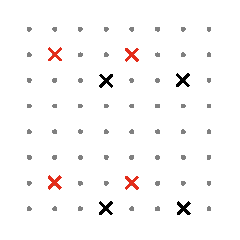
\includegraphics[width=3.5cm]{figures_cachees}
  \end{minipage} \\
\begin{enumerate}
 \item La face de devant sur la première figure ;
 \item La face de derrière sur la deuxième figure.
 \end{enumerate}
\end{exercice}


\begin{exercice}[Triangles particuliers]
\begin{minipage}[c]{0.38\linewidth}
On a représenté ci-contre un cube d'arête 4,5 cm.
 \end{minipage} \hfill%
 \begin{minipage}[c]{0.58\linewidth}
  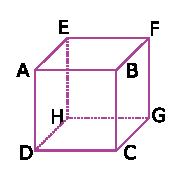
\includegraphics[width=2.5cm]{triangleBFG}
  \end{minipage} \\
\begin{enumerate}
 \item Quelle est dans la réalité la nature du triangle $BFG$ ? Justifie.
 \item Quelle est dans la réalité la nature du triangle $GBD$ ? Justifie.
 \item Construis ces deux triangles en vraie grandeur.
 \end{enumerate}
\end{exercice}


\begin{exercice}[Triangles particuliers (bis)] \label{VolSol_approf1}
$ABRINEUF$ est un pavé droit représenté ci‑après en perspective cavalière. On donne $BR = 7 \text{cm}$ et $AN = AB = 4 \text{cm}$.
 \begin{center} 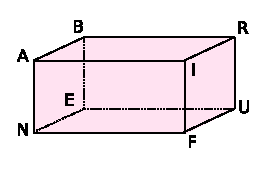
\includegraphics[width=4cm]{abrineuf} \end{center}
 \begin{enumerate}
  \item Quelle est dans la réalité la nature :
  \begin{itemize}
   \item du triangle $ABI$ ?
   \item du triangle $BIN$ ?
    \end{itemize}
Justifie tes réponses.
 \item Construis ces deux triangles en vraie grandeur.
 \end{enumerate}
\end{exercice}


\begin{exercice}[Se méfier des apparences]
On considère le parallélépipède rectangle de l'exercice \ref{VolSol_approf1}.
\begin{enumerate}
 \item Nomme deux arêtes qui sont perpendiculaires dans la réalité, mais pas sur le dessin.
 \item Peux‑tu répondre à la même question en remplaçant le mot « perpendiculaires » par « parallèles » ?
 \end{enumerate}
\end{exercice}


\begin{exercice}[Vrai ou faux ?]
On considère le parallélépipède rectangle de l'exercice \ref{VolSol_approf1}.
\begin{enumerate}
 \item Que peux-tu dire :
 \begin{itemize}
  \item des droites $(AN)$ et $(AI)$ ?
  \item des droites $(AB)$ et $(AI)$ ?
  \end{itemize}
 \item Que penses‑tu alors de l'affirmation : « Si deux droites sont perpendiculaires à une même droite alors elles sont parallèles. » ?
 \end{enumerate}
\end{exercice}


\begin{exercice}[Belle perspective]
\begin{minipage}[c]{0.44\linewidth} 
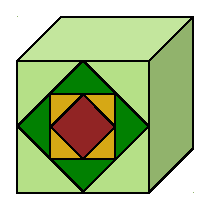
\includegraphics[width=3.2cm]{motif_persp}
 \end{minipage} \hfill%
 \begin{minipage}[c]{0.52\linewidth}
\begin{enumerate}
 \item Reproduis le cube ci‑contre en perspective cavalière sur papier quadrillé.
 \item Reproduis sur chaque face visible le motif figurant sur la face de devant.
 \end{enumerate}
  \end{minipage} \\
\end{exercice}


\begin{exercice}[La bonne marche à suivre]
\begin{minipage}[c]{0.52\linewidth} 
En collant des blocs cubiques identiques de 40 cm d'arête, on a construit un escalier comprenant quatre marches. Cet escalier doit ensuite être verni.
 \end{minipage} \hfill%
 \begin{minipage}[c]{0.44\linewidth}
 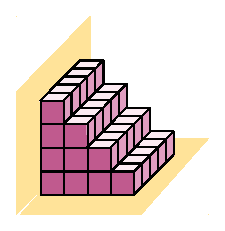
\includegraphics[width=3.2cm]{suivre_marche}
  \end{minipage} \\
\begin{enumerate}
 \item Combien de cubes constituent l'escalier ?
 \item Combien de faces carrées vont être vernies, sachant qu'on ne vernit pas la partie en contact avec le sol ou avec le mur ?
 \item Un pot de 1 L de vernis couvre 15 m\up{2}. Combien faudra‑t‑il de pots pour passer deux couches sur l'escalier ? 
 \item Calcule le nombre de cubes nécessaires à la fabrication d'un escalier semblable mais comprenant 100 marches.
 \end{enumerate}
\end{exercice}

%%%%%%%%%%%%%%%%%%%%%%%%%%%%%%%%%%%
%%%%%%%%%%%%%%%%%%%%%%%%%%%%%%%%%%%
%MiseEnPage
%%%%%%%%%%%%%%%%%%%%%%%%%%%%%%%%%%%
\newpage
%%%%%%%%%%%%%%%%%%%%%%%%%%%%%%%%%%%
%%%%%%%%%%%%%%%%%%%%%%%%%%%%%%%%%%%

\begin{exercice}[Des dés]
\begin{minipage}[c]{0.78\linewidth} 
Sur un dé à jouer, la somme des nombres de points inscrits sur deux faces opposées est égale à 7.
 \end{minipage} \hfill%
 \begin{minipage}[c]{0.18\linewidth}
 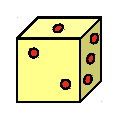
\includegraphics[width=1.5cm]{des1}
  \end{minipage} \\
\begin{minipage}[c]{0.78\linewidth} 
\begin{enumerate}
 \item Construis un patron du dé ci‑dessus puis marque les points sur chaque face.
 \item Sachant que le dé est à présent posé sur la face à trois points, combien de points comporte la face du dessus ? Et la face de droite ?
 \end{enumerate}
 \end{minipage} \hfill%
 \begin{minipage}[c]{0.18\linewidth}
 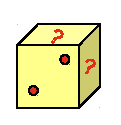
\includegraphics[width=1.5cm]{des2}
  \end{minipage} \\
\end{exercice}


\begin{exercice}[Patron]
On donne ci‑dessous la vue de face et la vue de côté d'un solide composé de deux parallélépipèdes rectangles accolés :
\begin{enumerate}
 \item Donne les dimensions de chaque parallélépipède rectangle.
 \item Fais un patron de chacun d'entre eux.
 \end{enumerate}
\begin{center} 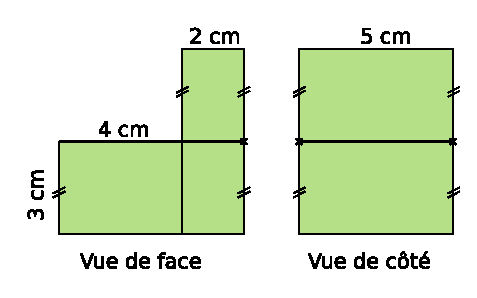
\includegraphics[width=8cm]{dim_patron} \end{center}
\end{exercice}


\begin{exercice}[Un solide peut en cacher un autre]
On considère un cube de 5 cm d'arête :
\begin{enumerate}
 \item Sur papier quadrillé, trace une représentation en perspective cavalière de ce cube puis marque les milieux des arêtes de la face de « dessus » et de la face de « dessous ».
 \item Décris le solide obtenu en reliant les huit points que tu as marqués. Fais‑en un patron.
 \item Que se passe‑t‑il si on recommence le processus ?
 \end{enumerate}
 \begin{center} 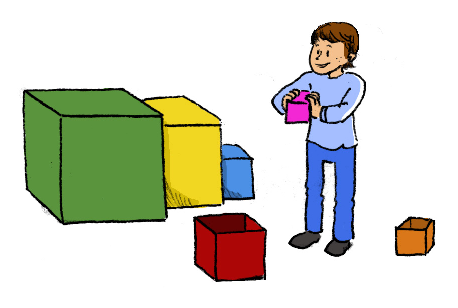
\includegraphics[width=5cm]{cube_cacher} \end{center}
\end{exercice}


\begin{exercice}[Chasse d'eau]
Un réservoir de chasse d'eau a la forme d'un pavé droit de 30 cm de longueur, 24 cm de largeur et 18 cm de hauteur. Il est rempli aux trois quarts de sa hauteur. Combien de litres d'eau sont utilisés lorsqu'on tire cette chasse d'eau ?
\end{exercice}


\begin{exercice}[Cube percé]
Calcule le volume de ce solide qui est un cube percé de part en part au centre de chaque face :
 \begin{center} 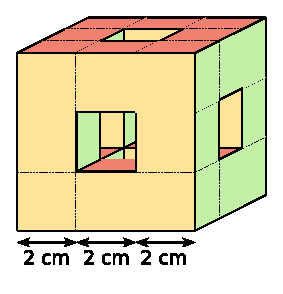
\includegraphics[width=4.5cm]{cube_perce} \end{center}
\end{exercice}


\begin{exercice}[Des pièces]
Les figures ci‑dessous représentent deux pièces d'un jeu. Compare leurs volumes respectifs :
 \begin{center} 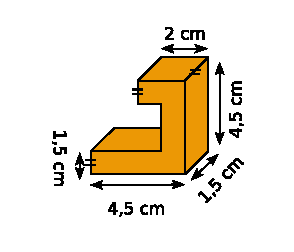
\includegraphics[width=4.5cm]{pieces_jeu1} \end{center}
 
 \begin{center} 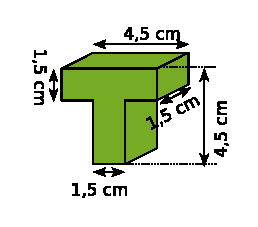
\includegraphics[width=4.5cm]{pieces_jeu2} \end{center}
\end{exercice}



